\documentclass[compress,11pt]{beamer}
%\includeonly{pendel}
\usetheme{Ilmenau}
%\usetheme{fau-4-3}
%\usecolortheme{beaver}
%\beamertemplatenavigationsymbolsempty
\usepackage[ngerman]{babel}
\usepackage{marvosym}
\usepackage{multimedia}
\usepackage[utf8]{inputenc}
\usepackage{amsmath}
\usepackage{amsfonts}
\usepackage{amssymb}
\usepackage{graphicx}
\usepackage{esvect}
%\author{}
\title{EP Gruppe 8}
%\setbeamercovered{transparent}
%\setbeamertemplate{navigation symbols}{}
%\logo{}
%\institute{}
%\date{}
%\subject{}
\usepackage{verbatim}
\begin{document}
\section{Einführung in PID-Regelung}
\subsection{Übersicht über Regelungstypen}
\subsubsection{I-Regler}
\begin{frame}
Übertragungsgleichung:
\begin{equation}
u(t) = K_p \cdot e(t)
\end{equation}
Hierbei sind:
\begin{itemize}
\item $e(t)$: Regelabweichung des Systems (Differenz von Sollwert und Istwert der zu regelnden Größe, bei und die Temperatur)
\item $u(t)$: Stellgröße, die an die Regelstrecke weitergegeben wird, um der Regelabweichung entgegenzuwirken
\item $K_p$: Regler-Parameter, mit dem der Abweichung entgegengewirkt wird
\end{itemize}
\end{frame}
\begin{frame}
\begin{block}{Eigenschaften des P-Reglers}
\begin{itemize}
\item Regelung ist relativ schnell
\item Stellgröße kann schnell hohe Werte annehmen und damit an Begrenzungen des Systems stoßen
\item Sollwert nur durch P-Regelung nicht erreichbar, entweder Näherung von unten oder ungedämpfte Schwingung um die Stellgröße
\end{itemize}
\end{block}

$\Rightarrow$ P-Regler alleine werden nur selten in der Praxis verwendet

\end{frame}
\subsubsection{I-Regler}
\begin{frame}

Übertragungsgleichung:
\begin{equation}
u(t) = K_t \cdot \int_0^t e(\tau) \mathrm{d}x
\end{equation}
Hierbei sind:
\begin{itemize}
\item $e(t)$, $u(t)$ wie oben
\item $K_t$: Regler-Parameter, mit dem der Abweichung entgegengewirkt wird
\end{itemize}
\end{frame}
\begin{frame}
\begin{block}{Eigenschaften des I-Reglers}
\begin{itemize}
\item Regelung ist relativ schnell
\item Stellgröße kann schnell hohe Werte annehmen und damit an Begrenzungen des Systems stoßen
\item Sollwert nur durch P-Regelung nicht erreichbar, entweder Näherung von unten oder ungedämpfte Schwingung um die Stellgröße
\end{itemize}
\end{block}

\end{frame}

\begin{frame}


\subsection{Aufgabe a)}
%Schaltung
\begin{itemize}
\item Metallblock wurde mittels Peltierelement erwärmt
\item Widerstand des Blocks wurde gemessen und in Temeratur umgerechnet
\end{itemize}
Aufgabe war es, mittels Power-Supply den Strom am Peltierelement so zu regeln, dass die Temperatur des Blocks konstant bleibt
\end{frame}
\begin{frame}
\textsc{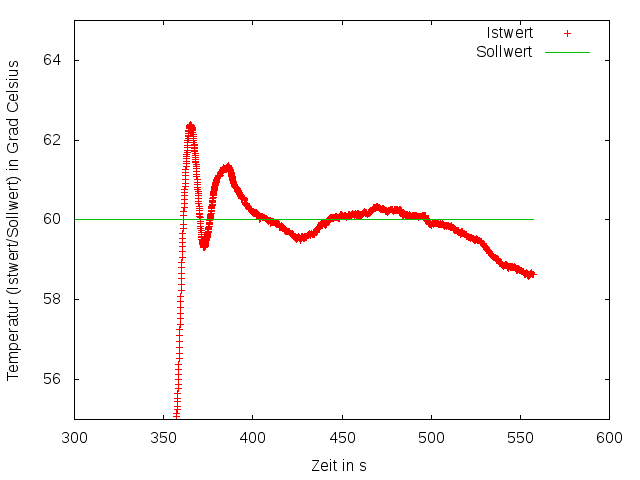
\includegraphics[width=.7\textwidth]{../2aufgabe/2a_T_genauer}\\}
Ergebnis der Regelung
\end{frame}
\begin{frame}
\begin{block}{"Vorgehensweise" beim Regeln}
\begin{itemize}
\item falls Temperatur zu niedrig $\Rightarrow$ mit Strom nachheizen
\item falls Temperatur zu hoch $\Rightarrow$ Strom abdrehen (Kühlung ja nicht möglich)
\item falls Sollwert bald erreicht wird $\Rightarrow$ Strom langsam herunterdrehen
\end{itemize}
\end{block}
\end{frame}



\subsection{Aufgabe b)}
\begin{frame}
Experiment wird nun mit automatisierter P-Regelung bei verschiedenen $K_p$-Parametern am Computer durchgeführt:\\

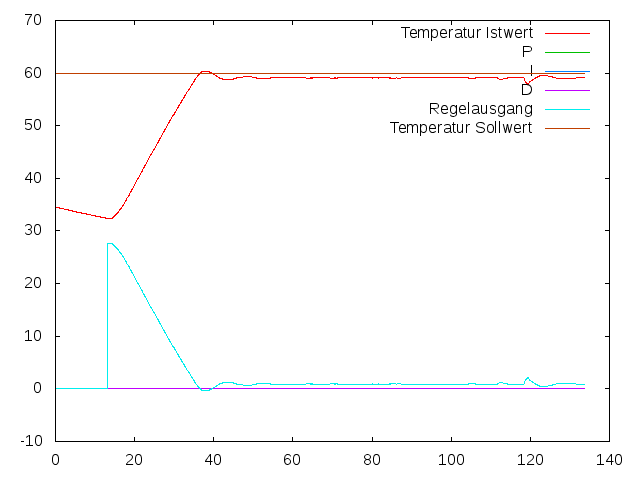
\includegraphics[width=.7\textwidth]{../2aufgabe/2bk1}\\
Regelung bei $K_p = 1$
\end{frame}
\begin{frame}

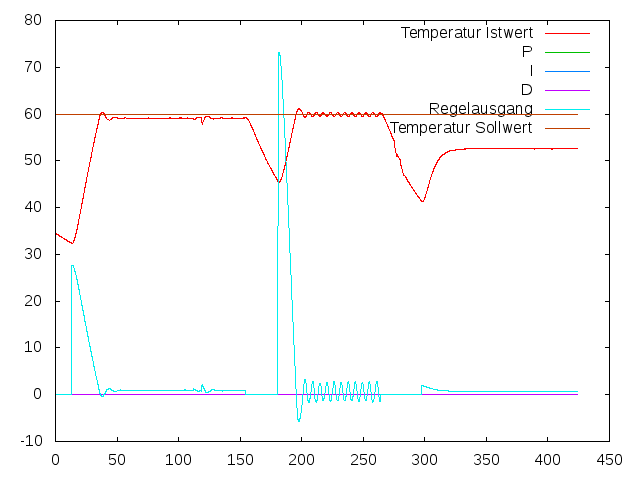
\includegraphics[width=.7\textwidth]{../2aufgabe/2bk,1}\\
Regelung bei $K_p = 0,1$
\end{frame}
\begin{frame}

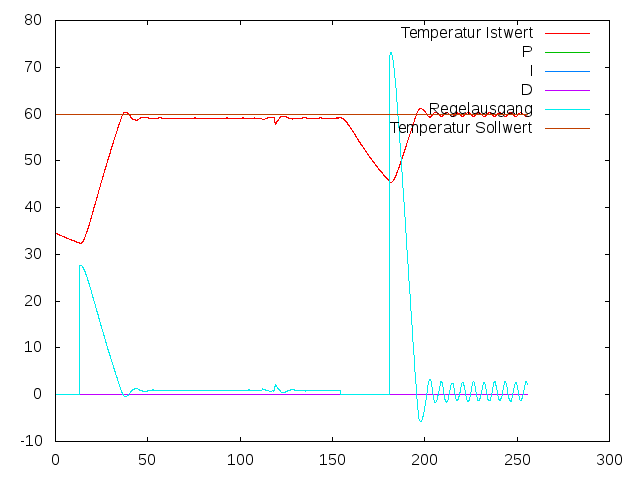
\includegraphics[width=.7\textwidth]{../2aufgabe/2bk5}\\
Regelung bei $K_p = 5$
\end{frame}
\begin{frame}
\begin{itemize}
\item Bei $K_p = 5$ wird keine konstante Temperatur erreicht, der Istwert osziliert ungedämpft um den Sollwert
\item Bei $K_p = 1$ und $0,1$ erreicht das System nicht den Sollwert, der Regler scheint zu schwach zu sein
\item Vergleich der Regler bei $K_p = 1$ und $0.1$ zeigt, dass die Regelgeschwindigkeit proportional zum Regelfaktor ist 
\end{itemize}
\end{frame}
\subsection{Aufgabe c) (I-Regler)}
\begin{frame}
\begin{itemize}
\item Abkühlung des Blockes auf ca. 50 $^\circ$ C
\item Dann I-Regelung der Temperatur mit $t_i = 100 s$
\end{itemize}
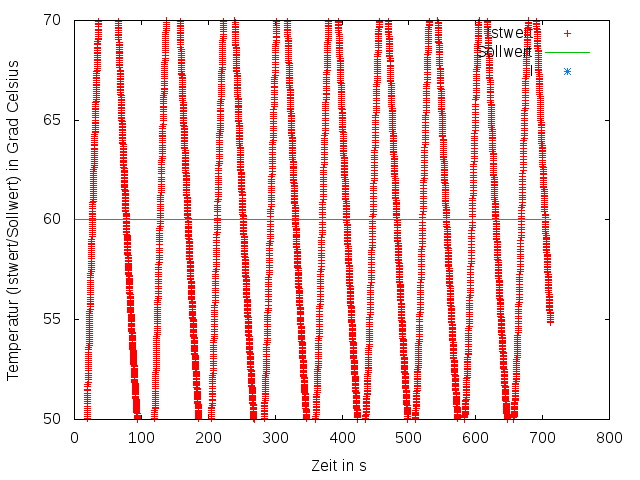
\includegraphics[width=.5\textwidth]{../2aufgabe/2c1}
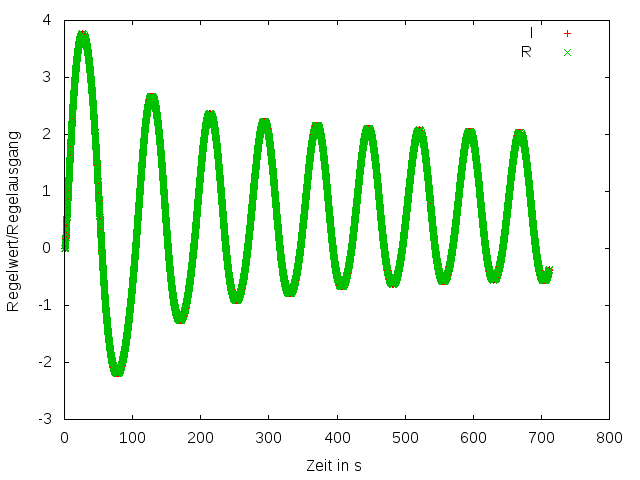
\includegraphics[width=.5\textwidth]{../2aufgabe/2c1_I}
\end{frame}
\begin{frame}
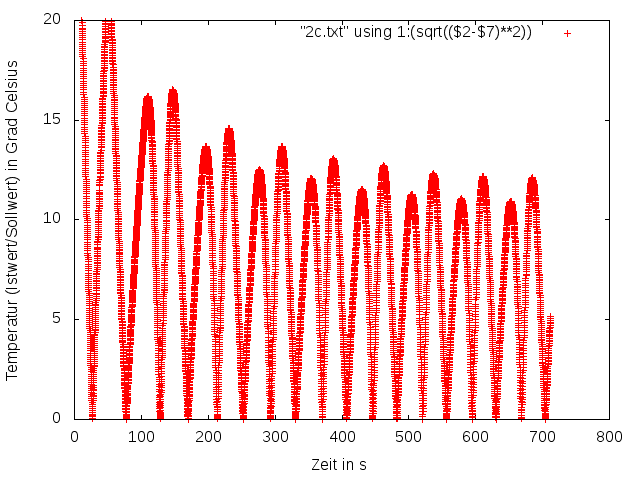
\includegraphics[width=.5\textwidth]{../2aufgabe/2c1_betrag}
\end{frame}




\begin{frame}
\begin{itemize}
\item Gleiche Messung wie eben
\item Es wurde allerdings "anti-windup-Funktion" verwendet
\end{itemize}
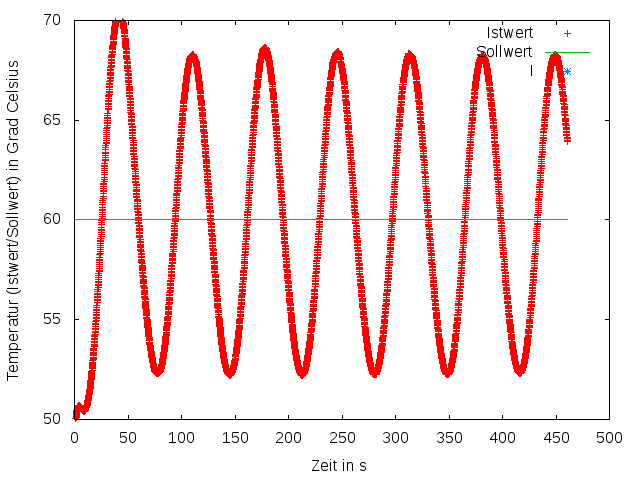
\includegraphics[width=.5\textwidth]{../2aufgabe/2c2}
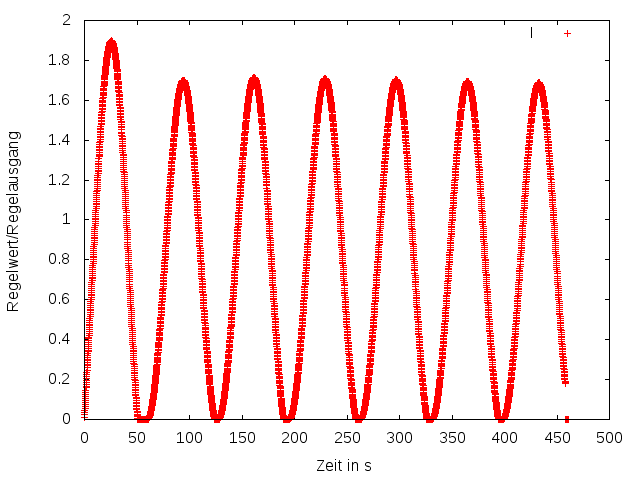
\includegraphics[width=.5\textwidth]{../2aufgabe/2c2_I}
\end{frame}
\begin{frame}
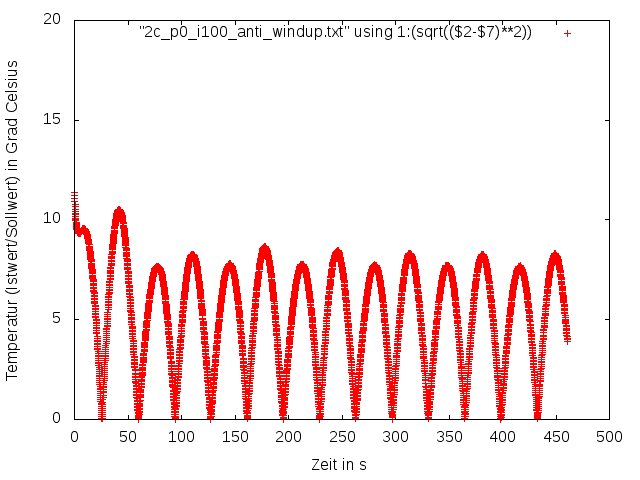
\includegraphics[width=.5\textwidth]{../2aufgabe/2c2_betrag}
\end{frame}
\begin{frame}
\begin{block}{Zur "anti-windup-Funktion"}
\begin{itemize}
\item Regelgröße berechnet sich bei uns durch $R = P + I + D$
\item falls $P + I + D > 2$ bzw. $P + I + D < 0$, wird $P + I + D = 2$ bzw. $= 0$ gesetzt
\item verhindert zu starken Ausschlag des Reglers und damit zu starke Oszilation der Ist-Wert-Kurve
\end{itemize}
\end{block}
\end{frame}


\begin{frame}
Grobe Abschätzunng des Zeitpunktes, an dem der I-Regler $T = 0$ wird:\\
Wähle Maxima der Oszilationen und fitte mit Gerade\\
$\Rightarrow$ Man erhält für die erste Messung:  $t_0 \approx 10280 s$\\
Und für die zweite:  $t_0 \approx 174212 s$
\begin{block}{Fazit}
I-Regelung ist in den meisten Fällen alleine nicht für den praktischen Gebrauch geeignet
\end{block}
\end{frame}
\subsection{PI-Regler}



\end{document}
